\message{ !name(examination.tex)}\documentclass[one column]{report}
\usepackage[utf8]{inputenc}

\usepackage{amsmath,amsthm,amssymb}

\usepackage{subcaption}
\usepackage{graphicx}

\usepackage{comment}

\usepackage{bm}
\renewcommand{\b}[1]{\bm{#1}}
\newcommand{\tr}{\text{ tr }}
\newcommand{\cov}[2]{\text{cov}(#1,#2)}
\newcommand{\corr}[2]{\text{corr}(#1,#2)}
\newcommand{\mean}[1]{\overline{\b{#1}}}
\usepackage{diagbox}
\newcommand{\abs}[1]{
  \left|
    #1
  \right|}
\newcommand{\rank}[1]{\text{rank #1}}
\newcommand{\diag}{\text{diag }}

\usepackage{biblatex}
\bibliography{ref}

\graphicspath{{./images/}}

\usepackage{listings}


\usepackage{color}

\definecolor{gray}{rgb}{0.5,0.5,0.5}
\definecolor{orange}{rgb}{0.8,0,0}

\lstdefinestyle{matlab}{
  belowcaptionskip=1\baselineskip,
  breaklines=true,
  frame=L,
  xleftmargin=\parindent,
  language=octave,
  showstringspaces=false,
  basicstyle=\footnotesize\ttfamily,
  keywordstyle=\bfseries\color{green},
  commentstyle=\color{gray},
  identifierstyle=\color{blue},
  stringstyle=\color{orange},
}
\lstdefinestyle{R}{
  belowcaptionskip=1\baselineskip,
  breaklines=true,
  frame=L,
  xleftmargin=\parindent,
  language=R,
  showstringspaces=false,
  basicstyle=\footnotesize\ttfamily,
  keywordstyle=\bfseries\color{green},
  commentstyle=\color{gray},
  identifierstyle=\color{blue},
  stringstyle=\color{orange},
}

\def\listingsfont{\ttfamily} 
\def\listingsfontinline{\ttfamily}

\title{TAMS39 - Examination exercises}
\author{Anton Karlsson\\antka388\\931217-7117}
\date{}
\begin{document}

\message{ !name(ex2.tex) !offset(-73) }
\section*{Exercise 2}
\label{sec:exercise-2}

\subsection*{(a)}
\label{sec:a-1}

The scatter plot can be found in Figure \ref{fig:ex2-scatter} the outlier can be
clearly be seen at $x_1 = 284$.
\begin{figure}[h]
  \centering
  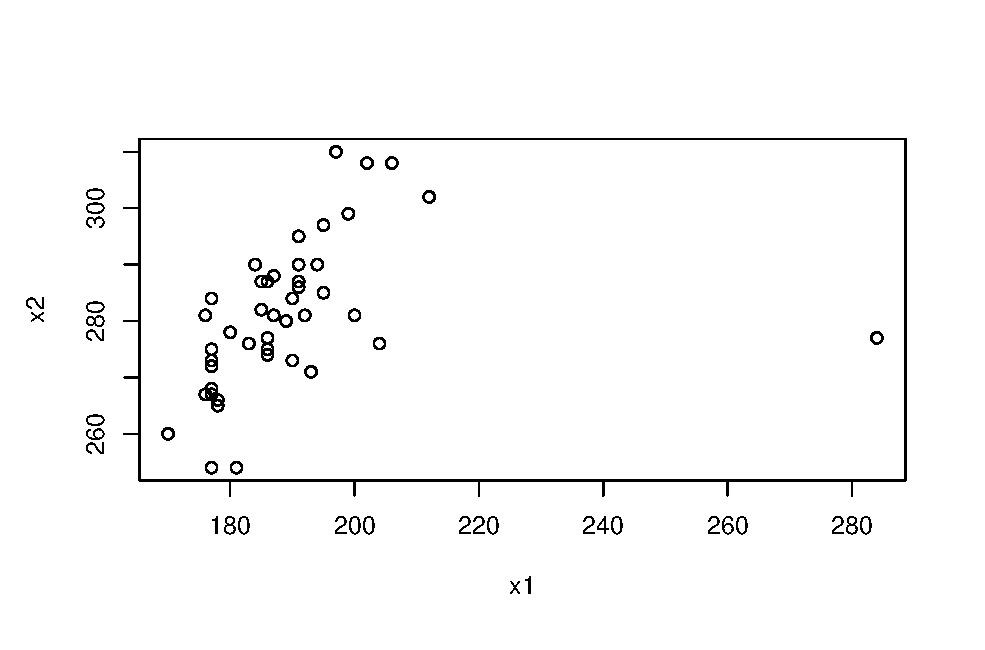
\includegraphics[width=5cm]{ex2-scatterplot}
  \caption{Scatter plot of the tail length and the wing span for male
    hook-billed kites.}
  \label{fig:ex2-scatter}
\end{figure}

\subsection*{(b)}
\label{sec:b-1}

We remove the sample with $x^{\rm male}_{1} = 284$.
Let $H_{0}: \b S_{\rm male} = \b S_{\rm female}$ versus $A \neq
H$. For this test we can use Box's test for equality of covariance
matrices, in which we reject $H_{0}$ if 
\begin{equation*}\label{eq:boxcorrection}
  (1 - u)
  \left(
    \left[
      \sum_{i=1}^{2}(n_{i} - 1)
    \right]
    \ln \abs{\b S_{\rm pooled}} - \sum_{i=1}^{2}(n_{i}-1) \ln \abs{\b S_{i}}
  \right) > \chi^{2}_{p(p+1)(g-1)/2}(1-\alpha),
\end{equation*}
where $p=2$ is the dimension of the populations, $g = 2$ is the
number of groups in the experiment, and
\begin{equation*}
  u = 
  \left[
    \sum_{i=1}^{2}\frac{1}{n_{i}-1} - \frac{1}{\sum_{i=1}^{2}(n_{i}-1)}
  \right]
  \left[
    \frac{2p^{2} + 3p - 1}{6(p+1)(g-1)}
  \right].
\end{equation*}
We represent the male population with $i=1$ and the female by
$i=2$. The covariance matrices $\b S_{i}$ is the sample mean for $i =
1,2$, and the pooled matrix, $\b S_{\rm pooled}$, is given by 
\begin{equation*}
  \b S_{\rm pooled}=  \frac{1}{\sum_{i=1}^{2}(n_{1} -
    1)}\sum_{i=1}^{2}(n_{i}-1)\b S_{i}  .
\end{equation*}
We get that 
\begin{equation*}
    (1 - u)
  \left(
    \left[
      \sum_{i=1}^{2}(n_{i} - 1)
    \right]
    \ln \abs{\b S_{\rm pooled}} - \sum_{i=1}^{2}[(n_{i}-1) \ln \abs{\b S_{i}}]
  \right) \approx 1.0431
\end{equation*}
and
\begin{equation*}
  \chi^{2}_{p(p+1)(g-1)/2}(1-\alpha) \approx 7.8147 , \quad \alpha =0.05.
\end{equation*}
Hence we should not reject $H_{0}$, the matrices can be pooled. On the
other hand, if we  instead change the outlier earlier to
$x_{1}^{\rm male} = 184$, we get that 
\begin{equation*}
    (1 - u)
  \left(
    \left[
      \sum_{i=1}^{2}(n_{i} - 1)
    \right]
    \ln \abs{\b S_{\rm pooled}} - \sum_{i=1}^{2}[(n_{i}-1) \ln \abs{\b S_{i}}]
  \right) \approx 1.2223,
\end{equation*}
and the same conclusion holds.
\subsection*{(c)}
\label{sec:c-1}
We remove the outlier.
 Using Result 6.2 in \cite[p. 286]{book} we can use the $T^{2}$ test
 where we accept $H_{0}:\b \mu_{\rm male} = \b \mu_{\rm female}$ versus
 $H_{1}:\b \mu_{\rm male} \neq \b \mu_{\rm female}$ if 
\begin{equation*}
T^{2} = \b Y^{T}
\left[
  \left(
    \frac{1}{n_{\rm male}} + \frac{1}{n_{\rm female}}
  \right)
  \b S_{\rm pooled}
\right]^{-1} \b Y
\leq \frac{(n-2)p}{n-1+p}F_{p, n-1+p}(1-\alpha) =:c^{2}_{\alpha},
\end{equation*}
with a confidence level of $1-\alpha$, where $\b Y = \b X_{\rm male}- \b
X_{\rm female} - (\mean X_{\rm male}- \mean X_{\rm female} )$ and $n$ is the total number of samples. From the given data, we get that
 $T^{2}\approx 24.96 $
and $c^{2}_{\alpha} \approx 6.28$, thus we reject $H_{0}$. \\
\\
If we instead change the outlier to 184, we get $T^{2} \approx 25.66$ and
$c_{\alpha}^{2} \approx  6.27$, so we get the same conclusion as when
we removed the outlier; $H_{0}$ is rejected.
\subsection*{(d)}
 From the remark found in \cite[p. 289]{book}, the linear combination
 $\b a^{T} (\mean x_{\rm male} - \mean x_{\rm female})$ with $\b a
 \propto \b S_{\rm pooled}^{-1}(\mean x_{\rm male} - \mean x_{\rm
   female}) =
 \begin{pmatrix}
   -0.16 &0.09
 \end{pmatrix}^{T}
$ is most responsible for rejecting $H_{0}$ in Exercise (c). 
\subsection*{(e)}
\label{sec:e}

The confidence region if given by the equation
\begin{align}
  \label{eq:ex2-conf-region}
 (\mean x_{\rm male}  - \mean x_{\rm female} - \b \mu)^{T}
\left[
  \left(
    \frac{1}{n_{\rm male}} + \frac{1}{n_{\rm female}}
  \right)
  \b S_{\rm pooled}
\right]^{-1} (\mean x_{\rm male}  - \mean x_{\rm female} - \b \mu) \nonumber
\\
\leq \frac{(n-2)p}{n-1+p}F_{p, n-1+p}(1-\alpha) =:c^{2}_{\alpha}
\end{align}
where for $\mu = (\mu_1, \mu_2)$, and $\alpha = 0.05$. The confidence
ellipse is represented in Figure \ref{fig:ex2fig}.

\begin{figure}[h]
  \centering
  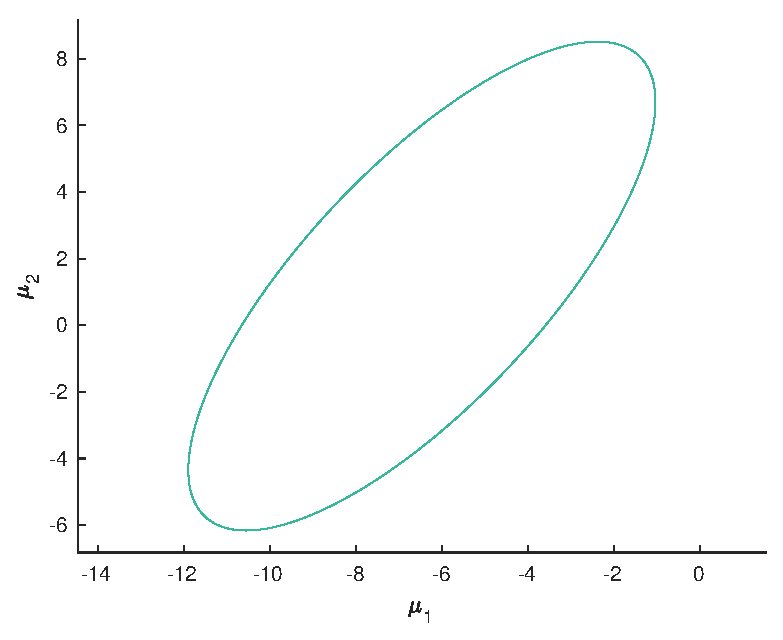
\includegraphics[width=10cm]{ex2fig}
  \caption{The confidence region of the difference
    $\b \mu_{\rm male} - \b \mu_{\rm female}$ with confidence 95\%. }
  \label{fig:ex2fig}
\end{figure}
The simultaneous confidence interval are $\b \mu = \b \mu_{\rm male}- \b
\mu_{\rm female}$ then we get that the confidence region for $\mu_{1}$
is given by 
\begin{equation*}
  \begin{pmatrix}
   -11.90 &-1.03  
  \end{pmatrix}
\end{equation*}
and, for $\mu_{2}$, 
\begin{equation*}
  \begin{pmatrix}
   -6.16 &8.52  
  \end{pmatrix}.
\end{equation*}
The confidence intervals ''frames'' the confidence region, as is shown
in Figure \ref{fig:ex2_sim_intervals}. 
\begin{figure}[h]
  \centering
  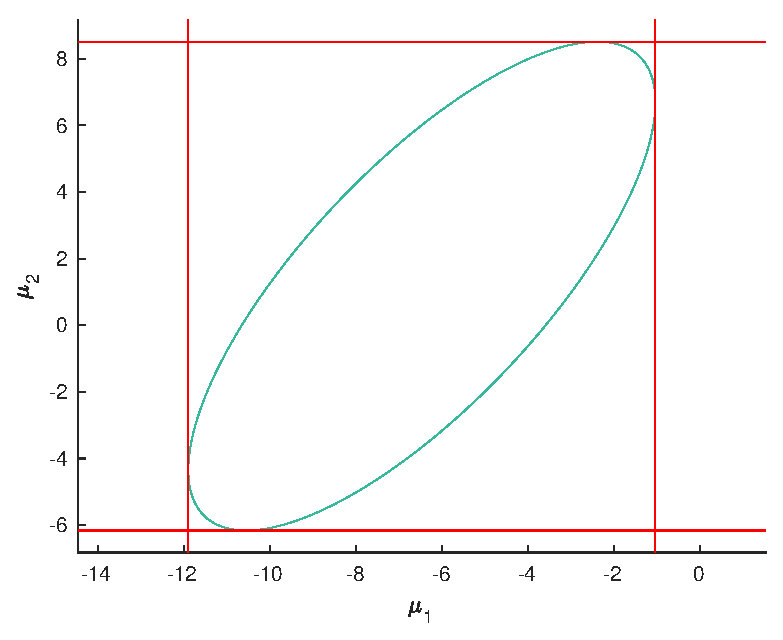
\includegraphics[width=10cm]{ex2fig_with_sim_intervals}
  \caption{Confidence region with and the simultaneous $T^{2}$-intervals plotted. }
  \label{fig:ex2_sim_intervals}
\end{figure}
\subsection*{(f)}
\label{sec:f}
There is evidence for that female birds have longer tails. However,
there is no significant difference between the genders when it comes to
the length of their wingspan. 


%%% Local Variables:
%%% mode: latex
%%% TeX-master: "examination"
%%% End:

\message{ !name(examination.tex) !offset(-159) }

\end{document}
%%% Local Variables:
%%% mode: latex
%%% TeX-master: t
%%% End:
